\documentclass{article}
\usepackage[utf8]{inputenc}
\usepackage{subfig}

%References
\usepackage{natbib}
%IMPORTANT use https://www.citationmachine.net/ if you need to generate references!
% \citep{reference} creates Harvard Style references throughout

%Colors
\usepackage{xcolor}

\usepackage[protrusion=true,expansion]{microtype}

%Code Markup
\usepackage[outputdir=cache]{minted}
%Syntax Highlighting Style
\definecolor{bggray}{RGB}{40,40,40}
\newmintedfile[javacode]{java}{
	style=fruity,
	bgcolor=bggray,
	linenos,
	breaklines,
	tabsize=2,
	obeytabs
}

%Page Margins and stuff
\usepackage{geometry}
 \geometry{
 a4paper,
 total={170mm,257mm},
 left=20mm,
 }

%Pictures
\usepackage{graphicx}
\graphicspath{ {./images/} }

%Move the title position
\usepackage{titling}

\setlength{\droptitle}{-8.5em} %Up, near the top but not too high

\title{Assignment 4 - CT213 Computer Systems \& Organization}
\author{Daniel Hannon (19484286)}
\date{November 2020}

\begin{document}
	\maketitle
	\section{Source Code}
	\begin{figure}[h!]
		\centering
		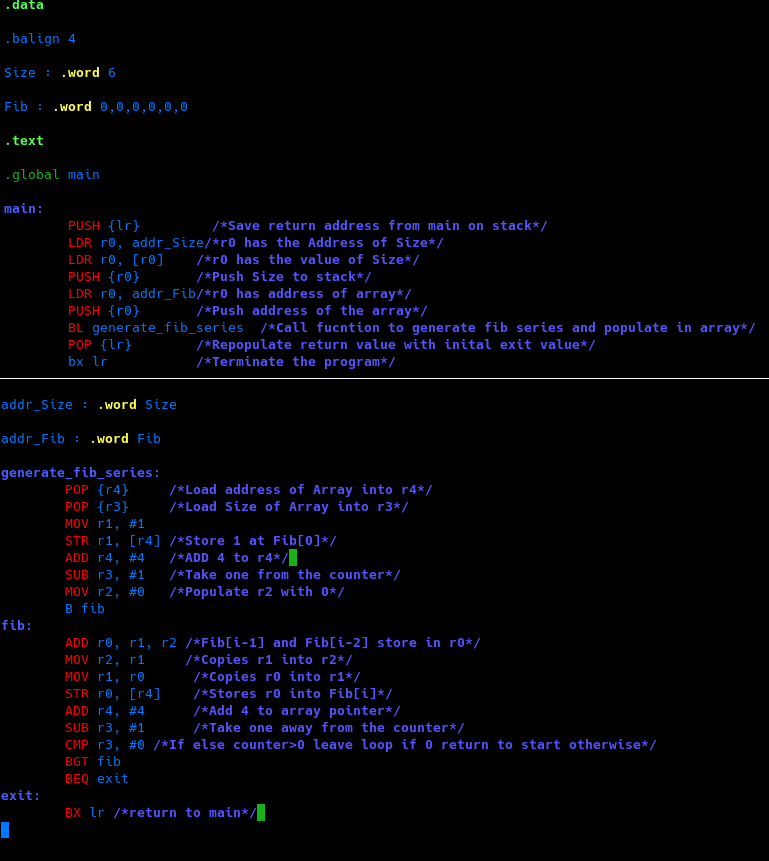
\includegraphics[width=\textwidth]{code.png}
	\end{figure}
	\newpage
	\section{GDB Screenshots}
	\subsection{First and Second Stack States}
	\begin{figure}[h!]
		\centering
		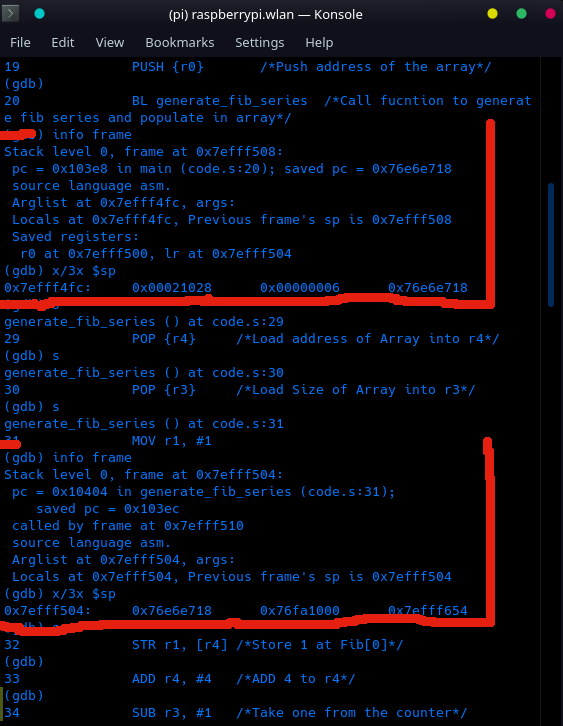
\includegraphics[width=\textwidth]{stack1_2.png}
	\end{figure}
	\newpage
	\subsection{Final Stack State and Array Values}
	\begin{figure}[h!]
		\centering
		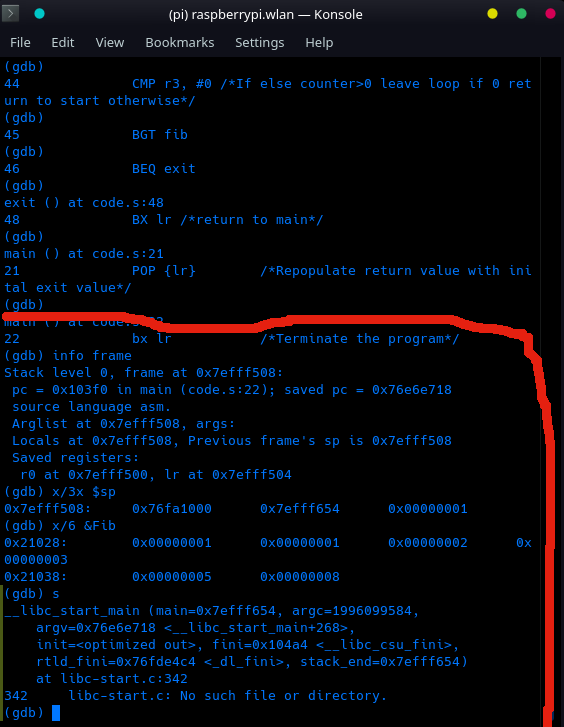
\includegraphics[width=\textwidth]{stack_final_fib_values.png}
	\end{figure}
	starting at the line with x/6 \&Fib the contents of the array are clearly shown 
	\newpage
	\section{Stack State Diagrams}
	\begin{tabular}{|c|c|}
		\hline
		\textbf{ADDRESS} & \textbf{VALUE} \\
		\hline
		0x7efff504 & lr \\
		\hline
		0x7efff500 & Count Value\\
		\hline
		\textbf{SP}0x7efff4fc & Fib pointer\\
		\hline
	\end{tabular}
	Immediately before function call\\ \\
	\begin{tabular}{|c|c|}
		\hline
		\textbf{ADDRESS} & \textbf{VALUE}\\
		\hline
		\textbf{SP} 0x7EFFF504 & Return Address\\
		\hline
		0x7EFFF500 & Old Count Value\\
		\hline
		0x7EFF4FC & Fib Address\\
		\hline
	\end{tabular}
	Immediately after the variables in the stack are unloaded \\
	\begin{tabular}{|c|c|}
		\hline
		\textbf{ADDRESS} & \textbf{VALUE} \\
		\hline
		\textbf{SP} 0x7EFFF508 & \\
		\hline
		0x7EFFF504 & Return Address\\
		\hline
		0x7EFFF500 & Old Count Value\\
		\hline
		0x7EFF4FC & Fib Address\\
		\hline
	\end{tabular}
	Final position of the stack pointer
	%Sets to Harvard Style and links the references file
	\bibliographystyle{agsm}
	\bibliography{references}
\end{document}